\documentclass[10pt,letterpaper]{article}
\usepackage[margin=0.78in]{geometry}
\usepackage[T1]{fontenc}
\usepackage{lmodern,microtype,graphicx,booktabs,tabularx,amsmath,amssymb,xcolor,fancyhdr,enumitem}
\usepackage[hyphens]{url}
\usepackage[colorlinks=true,linkcolor=teal,urlcolor=teal]{hyperref}
\definecolor{ink}{HTML}{243447}\definecolor{teal}{HTML}{006B72}
\setlength{\parindent}{0pt}\setlength{\parskip}{6pt}\setlist{nosep,leftmargin=1.5em}
\pagestyle{fancy}\fancyhf{}\fancyhead[L]{\small Closure-time summaries with unfinished requests}\fancyhead[R]{\small Independent study 05}\fancyfoot[C]{\thepage}\setlength{\headheight}{14pt}
\hypersetup{pdftitle={Closure-time summaries with unfinished requests},pdfauthor={Independent research program},pdfsubject={Captured NYC311 records, synthetic observation cutoffs and restricted recorded closure time}}
\begin{document}\color{ink}
{\LARGE\bfseries Closure-time summaries with unfinished requests\par}
{\large A finite-cohort NYC 311 reconstruction with explicit observation bounds\par}
\textbf{Independent research study 05}\hfill29 October 2026\\
AI-assisted analysis and manuscript. Not peer reviewed or accepted for formal publication.

\section*{Decision and verified finding}
An average calculated only from completed service requests can describe a faster-moving subset of a recent cohort. A decision-useful closure-time summary needs a fixed request cohort, a stated observation window and an explicit definition of closure. Omitting unfinished requests can change the summary even when every completed request is measured correctly.

This study uses 273,641 captured NYC 311 requests across three agency codes and four creation cohorts in 2026. After 195 backward-date records are quarantined under a fixed quality rule, 273,446 requests remain eligible. We reconstruct two earlier observation cutoffs on these later records. These are synthetic observation rules on real administrative data, not historical dashboard exports.

In the primary held comparison---eight panels, a 28-calendar-day restricted horizon, cutoff 35 days after cohort start and the recorded-date endpoint---the censoring-aware restricted mean has an equal-panel mean absolute error of 0.033 days against the later captured-record benchmark. The fair, capped completed-case-only summary has an error of 1.689 days. The restricted mean is closer in all eight panels. Across all 96 predeclared held endpoint/cutoff/horizon comparisons, it is closer in every comparison; all results remain available.

\begin{center}\begin{tabularx}{\linewidth}{Xr}\toprule
Primary comparison against the later recorded-date benchmark & Calendar days\\\midrule
Mean absolute error, censoring-aware restricted mean & 0.033\\
Mean absolute error, capped completed-case summary & 1.689\\
Held panels favoring the restricted mean & 8 / 8\\\bottomrule
\end{tabularx}\end{center}

\textbf{Practical recommendation.} Report a fixed-horizon, all-request cohort summary alongside the unfinished fraction and observation bounds. If a product-limit estimate is used, state its censoring assumptions and check their plausibility as calendar cohorts change. Retain a completed-case average as a labeled subset description rather than treating it as the cohort's waiting-time estimate. A prospective dashboard needs dated exports and an audited endpoint before operational claims are made.

\textbf{Important limits.} The benchmark is the later recorded closure date, not verified problem resolution, first closure or a complete reopening history. Current status is available only in the later capture. NYC's terms state that older versions are not retained [2]. Source consistency checks do not establish historical availability, and these selected panels do not establish future agency performance, causal improvement or realized public benefit. The censoring assumptions remain unverified.

\clearpage
\section*{1. Source, partitions and quality accounting}
We retrieve the official 2020--present NYC 311 dataset, endpoint \texttt{erm2-nwe9} [1]. The fixed panel includes all requests with creation day 1--28 in April, May, June or July 2026 and agency code DOT, DEP or DSNY. This is a complete extraction of those filters, not a random sample or the city's entire service workload. Agency codes are source labels; different request mixes prevent a causal agency comparison.

Only \texttt{unique\_key}, \texttt{created\_date}, \texttt{closed\_date}, \texttt{agency} and \texttt{status} are requested. Sequential pages of 5,000 are ordered by unique key. All twelve initial and final coverage counts match; both metadata reads report \texttt{rowsUpdatedAt=1793237699}. The capture date is 29 October 2026. Global ID uniqueness, requested field scope and every public aggregate cell are independently checked. Stable metadata/counts provide bounded capture evidence, not an atomic-transaction guarantee.

\begin{center}\small\begin{tabular}{lllrrr}\toprule
Agency & Cohort & Partition & Source & Quarantined & Eligible\\\midrule
DOT & Apr & Development & 25,983 & 35 & 25,948\\
DEP & Apr & Development & 15,056 & 0 & 15,056\\
DSNY & Apr & Evaluation & 23,651 & 0 & 23,651\\
DOT & May & Development & 22,169 & 37 & 22,132\\
DEP & May & Development & 18,398 & 14 & 18,384\\
DSNY & May & Evaluation & 23,683 & 0 & 23,683\\
DOT & Jun & Evaluation & 22,180 & 66 & 22,114\\
DEP & Jun & Evaluation & 18,969 & 11 & 18,958\\
DSNY & Jun & Evaluation & 26,399 & 0 & 26,399\\
DOT & Jul & Evaluation & 21,991 & 20 & 21,971\\
DEP & Jul & Evaluation & 28,259 & 12 & 28,247\\
DSNY & Jul & Evaluation & 26,903 & 0 & 26,903\\
\bottomrule\end{tabular}\end{center}

Development uses DOT/DEP in April/May; the other eight panels are held evaluation. All source inputs, quality counts and current-status coherence were visible before the code freeze; inputs were not blinded. Held survival, restricted means and benchmark errors were computed after the public twenty-dependency freeze at revision \texttt{13f67e0}. No endpoint, horizon or cutoff was chosen from held errors.

The 195 excluded records have closure datetimes earlier than creation. Each panel passes the predeclared exclusion cap of 0.5\% and minimum of 100 eligible requests. There are no other quarantined closure-quality categories in this capture. Among eligible records, 392 have a valid closure date with a current status other than Closed; one has Closed status without a date. Both counts are retained rather than silently repaired.

\textbf{Reuse and privacy.} The official FAQ allows reuse subject to portal terms [2]. Original minimized responses, identifiers, exact timestamps and raw status strings remain outside Git. Public cells contain only agency, cohort, creation-day index, recorded-delay cell, status category, quality code and count. Values 0--45 days are exact; longer delays are pooled as \texttt{gt45}, sufficient for every declared cutoff and horizon. No address, coordinate, problem type, narrative or requester information is retrieved. Third-party source documents are linked, not republished.

\clearpage
\section*{2. Fixed estimand and independent computation}
Use source floating calendar timestamps without inventing a timezone. A valid closure must not precede its creation datetime or exceed the capture date. The analyzed delay $T$ is the difference between closure and creation calendar dates, not elapsed hours, staff work time or customer experience. Same-day valid closure has delay zero.

The primary endpoint accepts a valid recorded closure date irrespective of current status. The sensitivity also requires current status exactly Closed, normalizing case and surrounding whitespace. Missing or rejected dates mean no recorded closure under that endpoint. Current status defines a retrospective sensitivity; it is not a feature asserted to have been known at the earlier cutoff.

For a request created on day index $a\in\{1,\ldots,28\}$, reconstruct censoring time $C=c-(a-1)$ with $c\in\{35,45\}$. Thus follow-up ranges from 8--35 or 18--45 calendar days. Observe an event if $T\leq C$, otherwise censor at $C$. Missing dates and pooled delays above 45 cannot generate an observed event. Event/censor ties retain both groups in the risk set for the event factor.
\[
n_d=\sum_i w_i\,1(X_i\geq d),\qquad
e_d=\sum_i w_i\,1(X_i=d,\delta_i=1),\qquad
\widehat S(d)=\prod_{j\leq d}\left(1-\frac{e_j}{n_j}\right).
\]
Here $w_i$ is an aggregate-cell count, $X_i=\min(T_i,C_i)$ and $\delta_i$ indicates an observed event. Exact rational arithmetic retains every factor. For fixed horizons $\tau\in\{7,14,28\}$,
\[
\widehat\mu_{\rm KM}(\tau)=\sum_{d=0}^{\tau-1}\widehat S(d),\qquad
\mu_{\rm later}(\tau)=\frac{1}{N}\sum_i w_i\min(T_i,\tau).
\]
Absent or longer recorded dates contribute $\tau$ to the later benchmark. A positive survival tail without risk support before a required day makes the restricted mean NOT\_ESTIMABLE; a zero tail can remain zero. All declared settings are estimable here. Fixed truncation and unsupported-tail cautions follow established survival methods [4,5]; no new estimator is proposed and R execution is not claimed.

\textbf{Fair comparator.} Compute the mean of $\min(T,\tau)$ among observed completed requests, and compare its absolute error with the same capped benchmark. The traditional uncapped completed mean is retained in the full exports as a descriptive quantity, but is not scored against a different target. There is no model search, random seed, learned feature preprocessing, threshold tuning or inferential sampling interval.

\textbf{Observation bounds.} Observed events contribute their known capped time to both bounds. Censored requests contribute $\min(C,\tau)$ to the lower and $\tau$ to the upper bound. The later benchmark lies within these conservative finite-cohort bounds in every setting. They are not asserted to be sharp for integer times, confidence intervals or bounds on true resolution. KM is checked against them without clipping. Its independent-censoring and stable closure-distribution assumptions are not verified and can fail as creation-day request mix or queue conditions change.

\clearpage
\section*{3. The primary held comparison}
The table retains every held panel. ``Unfinished'' means no event observed by the reconstructed cutoff, not necessarily a request that was open in an actual historical export. All quantities except counts and unfinished percentages are calendar days on the same 28-day restricted target. The bounds use only the reconstructed observations.

\begin{center}\small\setlength{\tabcolsep}{4pt}\begin{tabular}{lrrrrrl}\toprule
Panel & Eligible & Unfinished & Later & Completed & KM & Observation bounds\\\midrule
DEP Jun & 18,958 & 5.4\% & 3.654 & 2.458 & 3.682 & [3.319, 3.833]\\
DEP Jul & 28,247 & 3.5\% & 2.410 & 1.586 & 2.416 & [2.174, 2.511]\\
DOT Jun & 22,114 & 15.5\% & 7.083 & 3.840 & 7.189 & [6.047, 7.573]\\
DOT Jul & 21,971 & 18.9\% & 7.935 & 3.802 & 7.989 & [6.534, 8.366]\\
DSNY Apr & 23,651 & 4.0\% & 2.922 & 1.925 & 2.918 & [2.626, 2.969]\\
DSNY May & 23,683 & 4.0\% & 2.898 & 1.877 & 2.882 & [2.600, 2.927]\\
DSNY Jun & 26,399 & 4.0\% & 3.056 & 2.116 & 3.092 & [2.793, 3.156]\\
DSNY Jul & 26,903 & 4.9\% & 4.008 & 2.850 & 3.997 & [3.650, 4.093]\\
\bottomrule\end{tabular}\end{center}

\begin{center}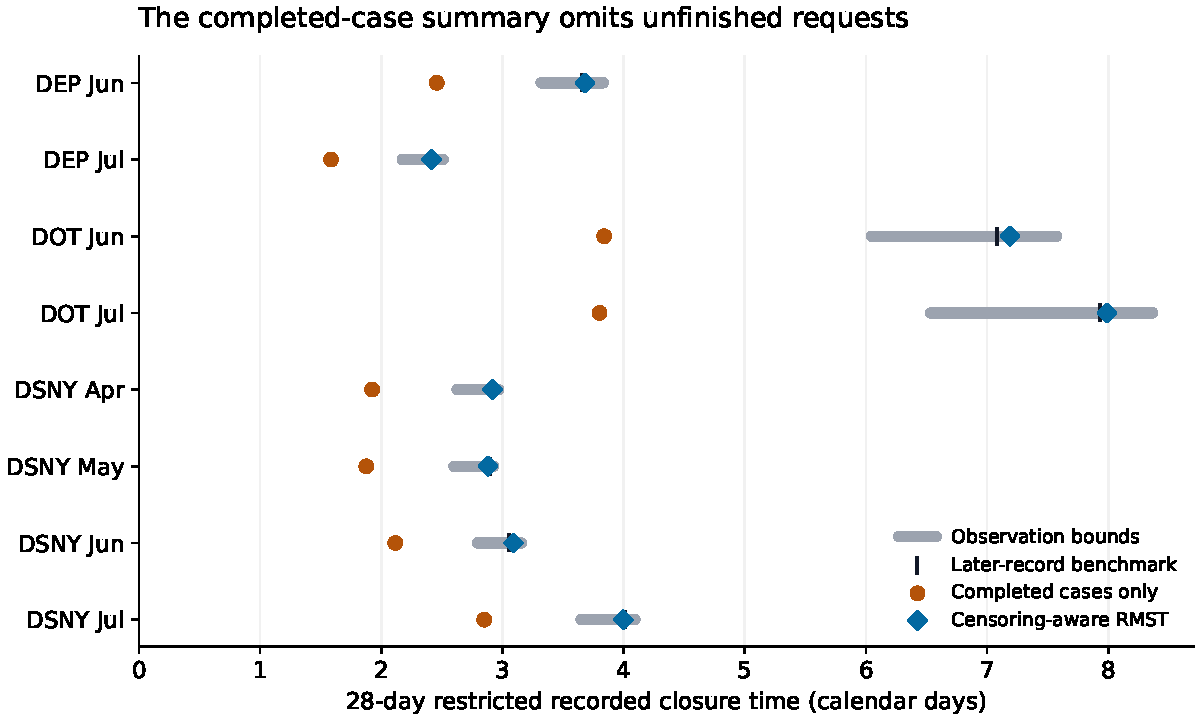
\includegraphics[width=\linewidth]{images/primary_comparison.pdf}\end{center}
{\small\textbf{Figure 1.} Recorded-date endpoint, cutoff +35, horizon 28; all cohorts are in 2026. Gray segments are observation bounds, black marks are the later benchmark, orange circles are capped completed-case means and blue diamonds are restricted means. Close benchmark/KM marks can overlap. These finite-panel bounds do not express uncertainty about problem resolution.}

The largest primary completed-case error occurs in DOT July: its capped subset mean is 3.802 days and the all-request later benchmark is 7.935 days; KM is 7.989 days. This descriptive contrast is sensitive to the request mix and the endpoint. It is not evidence that one agency, month or staffing practice is intrinsically better.

\clearpage
\section*{4. Survival curves and what early agreement means}
\begin{center}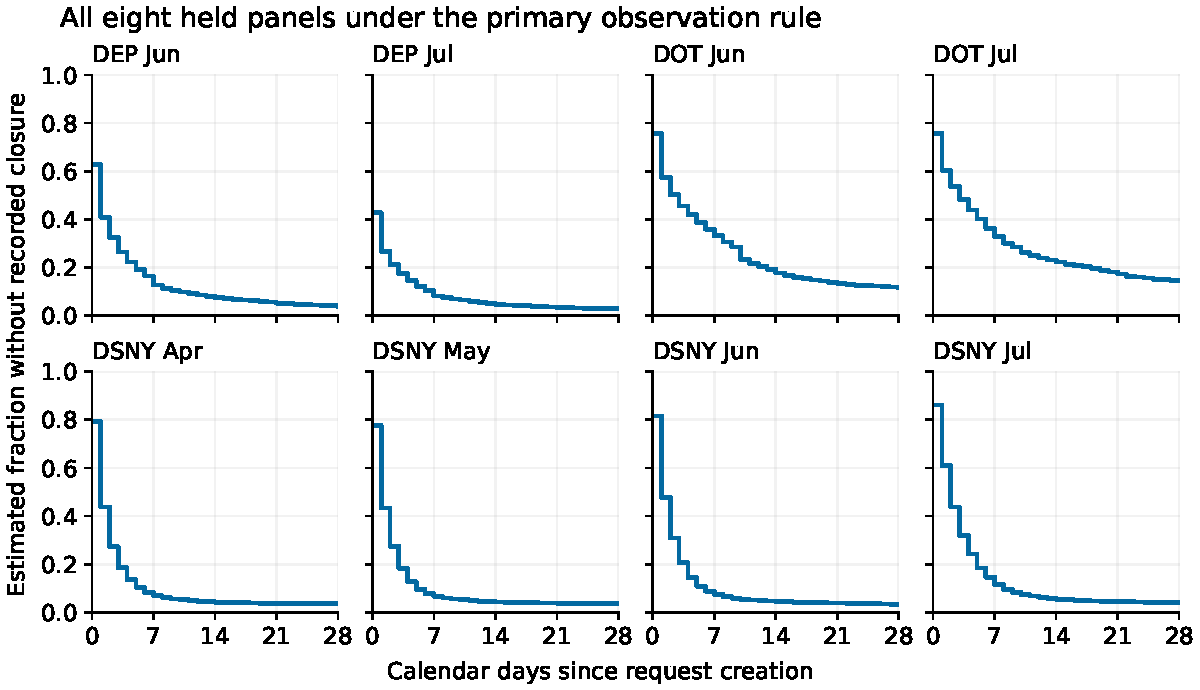
\includegraphics[width=\linewidth]{images/survival_overview.pdf}\end{center}
{\small\textbf{Figure 2.} All eight held product-limit curves for the primary date-only endpoint and cutoff +35, shown through day 28. Each curve is estimated under the same declared rule from weighted aggregate timing cells. The vertical scale is the estimated fraction without a recorded closure; it is not the fraction of customers with unresolved problems. All curves have risk support through the restricted horizon.}

The high early closure fractions, different same-day masses and later tails explain why a completed-case subset and an all-request target can be far apart. The curves preserve day-zero closures rather than forcing every request to wait a full day. They are descriptive reconstructions without confidence bands or causal comparisons between agencies.

\textbf{A structural check, not an extra validation claim.} Under cutoff +35, the shortest follow-up is eight days; under +45 it is eighteen. Consequently no request is censored before the full seven-day horizon, and under +45 none is censored before the full fourteen-day horizon. KM equals the later restricted benchmark exactly at those horizons by complete support. Their zero errors do not test recovery of an unobserved survival tail or establish robustness to dependent censoring. The 28-day comparison involves genuine reconstructed censoring within the horizon.

The completed-case comparator can still differ at an early horizon because it conditions on completion by the entire reconstructed cutoff. A request that would contribute a capped value to the cohort benchmark can be omitted from that completed subset. This is the denominator distinction the fair capped comparator is designed to expose.

\textbf{Endpoint sensitivity.} Requiring both current Closed status and a recorded date changes some eligible events. All date/status disagreements remain in the source accounting. The sensitivity is implemented for every panel, cutoff and horizon; it does not resolve whether the source date denotes first closure, whether a request reopened or whether the underlying problem was fixed. Only dated lifecycle records and endpoint review could establish those meanings.

\clearpage
\section*{5. Every held sensitivity result}
\begin{center}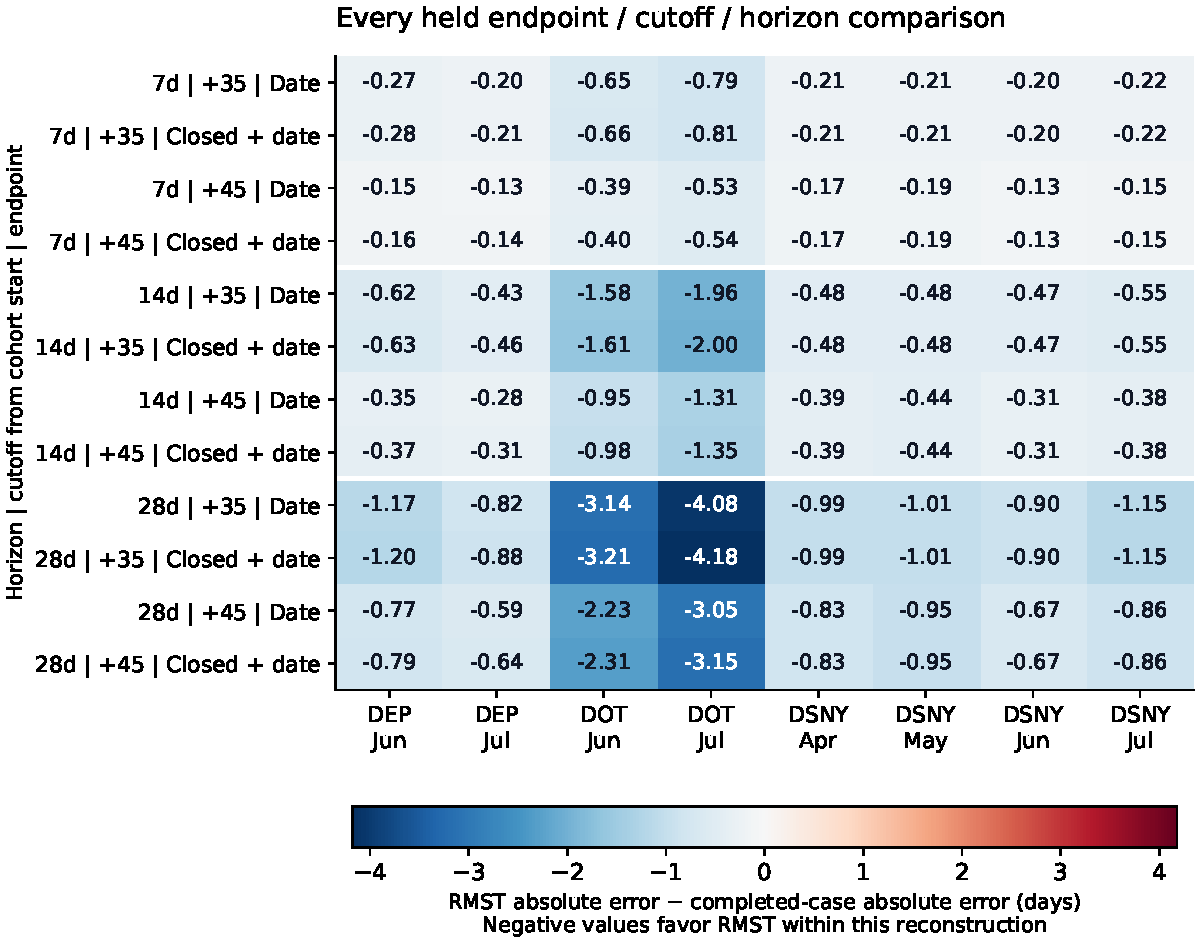
\includegraphics[width=\linewidth]{images/error_sensitivity.pdf}\end{center}
{\small\textbf{Figure 3.} All 96 held comparisons, arranged by the twelve fixed horizon/cutoff/endpoint settings and eight agency/cohort panels. Each cell is KM absolute error minus capped completed-case absolute error against that endpoint's later benchmark, in calendar days. Negative values favor KM. Colors share a symmetric zero-centered scale; values are rounded only for display. ``Date'' accepts the valid date alone; ``Closed + date'' also requires current Closed status. All panels are from 2026.}

No held setting is omitted or redefined after its result. Exact fractions, reported floating values, uncapped descriptive means, event/censor counts, survival support and bounds are retained in the public CSVs. The finite comparison does not assign a probability that the same ordering will hold in a new cohort or a prospective system.

\clearpage
\section*{6. Complete summaries, interpretation and next evidence}
Equal-panel mean absolute errors give each held agency/cohort panel the same weight; they do not weight by request count. Every setting has eight paired estimable panels, no ties and no KM estimate outside the observation bounds.

\begin{center}\small\begin{tabular}{rrlrrr}\toprule
Horizon & Cutoff & Endpoint & KM MAE & Completed MAE & KM closer\\\midrule
7 & 35 & Date & 0.0000 & 0.3447 & 8 / 8\\
14 & 35 & Date & 0.0020 & 0.8226 & 8 / 8\\
28 & 35 & Date & 0.0325 & 1.6889 & 8 / 8\\
7 & 35 & Closed + date & 0.0000 & 0.3503 & 8 / 8\\
14 & 35 & Closed + date & 0.0021 & 0.8365 & 8 / 8\\
28 & 35 & Closed + date & 0.0323 & 1.7211 & 8 / 8\\
7 & 45 & Date & 0.0000 & 0.2290 & 8 / 8\\
14 & 45 & Date & 0.0000 & 0.5524 & 8 / 8\\
28 & 45 & Date & 0.0055 & 1.2488 & 8 / 8\\
7 & 45 & Closed + date & 0.0000 & 0.2346 & 8 / 8\\
14 & 45 & Closed + date & 0.0000 & 0.5659 & 8 / 8\\
28 & 45 & Closed + date & 0.0056 & 1.2803 & 8 / 8\\
\bottomrule\end{tabular}\end{center}

The small 28-day KM errors here are empirical results, not a guarantee of unbiasedness. The fixed end-of-cohort cutoff gives later creation days less follow-up. If those days also carry different request types, calendar effects or closure processes, censoring can depend on closure time. A single later capture cannot establish the required independence. Longer follow-up and a consistent endpoint help define the target, but cannot recover missing lifecycle history.

The benchmark is mature relative to each declared 28-day horizon: even the last July creation date is more than 28 days before capture. Dates beyond the horizon or missing under the endpoint contribute the cap. This defines a fully observed \emph{captured-record} target; it does not turn absent dates into confirmed unresolved problems. Later source revisions can change this target. The portal warns that corrections and refreshed values may replace earlier records [2].

The practical use is a measurement check for dashboard designers: expose cohort membership, unfinished counts, follow-up support and the restricted horizon before presenting a mean as performance. Avoid treating cross-agency differences as causal or attributing a reduction in this summary to an intervention. No deployed service system, adopted workflow, customer outcome or saving is established.

\textbf{Smallest next evidence.} Preserve regular dated minimal exports; audit the interpretation of closure and reopening on an authorized sample; evaluate creation-day/request-mix dependence and missing-date mechanisms; then predeclare an untouched future cohort. A prospective comparison should retain the same fair capped target and report failures as well as successes. This study does not authorize or claim that work.

\clearpage
\section*{7. Reproduction and independent evidence}
The repository contains aggregate source cells, query/page hashes, normalized timing cells, the fixed protocol, complete results, figures and this manuscript. It does not contain minimized raw requests or third-party source documents. Private-original reconciliation checked 1,368,205 selected fields and 69,874 aggregate scalar values. Public replay checks the aggregate source independently of live service access; it cannot reproduce the unpublished identifiers and exact timestamps.

Fourteen boundary fixtures cover source privacy/cohort behavior, same-day events, event/censor ties, a hand-computable curve, unsupported positive tails, zero survival, endpoint differences and capped targets. Development/evaluation verification checks 11,040 exact scalars, 3,408 reported floats and 2,112 separate decimal values. SQL constructs observation/risk/event/censor and benchmark sums; independently reduced integer products and 90-digit decimal integration reconstruct the curves. Decimal agreement tolerance is $10^{-70}$ and reported-float tolerance $10^{-12}$, fixed before held evaluation. These are arithmetic checks, not assumptions tests.

Isolated public replay matches 97,920 CSV fields or JSON documents exactly, with twenty frozen dependency hashes. Figure verification checks 368 plotted values. PDF text, numeric tables, complete commands, approved hashes, active-content exclusions and every rendered page are checked separately. The finite checks establish their stated scope, not universal correctness or accessibility conformance. Remote CI and release state are reported by the repository receipts rather than presumed by this manuscript.

\begin{verbatim}
python -m pip install -r requirements.txt
python -m unittest discover -s tests -v
python src/check_reproduction.py
python src/verify_figures.py
python src/verify_paper.py
python src/verify_public_package.py
\end{verbatim}
Python 3.10 is the declared replay runtime. NumPy 2.2.5, Matplotlib 3.10.9 and pypdf 6.10.0 are pinned; survival arithmetic uses Python integers/fractions and SQLite, without unnecessary machine learning. R manuals are method references only. Original source retrieval is a separate minimized-data operation with source/version gates; the commands above require no network after dependency installation.

\subsection*{Primary sources and method references}
{\footnotesize
[1] NYC Open Data. \href{https://data.cityofnewyork.us/Social-Services/311-Service-Requests-from-2020-to-Present/erm2-nwe9}{311 Service Requests from 2020 to Present}; \href{https://data.cityofnewyork.us/api/views/erm2-nwe9.json}{machine-readable schema}. Capture: 29 October 2026.\par
[2] NYC Open Data. \href{https://www.nyc.gov/opendata/get-started/FAQs}{Official FAQ}; \href{https://data.cityofnewyork.us/stories/s/Terms-of-Use/k9k7-3cje}{portal terms of use}. Reuse, agency authority, revisions, no retained older versions and warranty limits.\par
[3] NYC Open Data. \href{https://www.nyc.gov/opendata/news/all-news/311-Service-Requests-Updates}{311 dataset updates}; Socrata \href{https://dev.socrata.com/foundry/data.cityofnewyork.us/erm2-nwe9}{official endpoint documentation}. Unused problem/location fields remain excluded.\par
[4] R survival package. \href{https://stat.ethz.ch/R-manual/R-devel/library/survival/html/print.survfit.html}{Restricted mean and fixed truncation documentation}. Established methodology; no R execution claim.\par
[5] R survival package. \href{https://stat.ethz.ch/R-manual/R-devel/library/survival/html/summary.survfit.html}{Curve summary and unsupported extension cautions}.\par
}
\end{document}
